
\chapter{Introduction}

\vspace{-20pt}

I am proud to finally, officially introduce the world to \emph{Skedge}, a website I have been developing since December 2013. It began as a weekend project after I spent too much time trying to find interesting elective classes, and it wasn't until I briefly presented it at a RocHack ``Hacker Night'' when I realized the potential it had to help others as well. I never expected the subject of my senior thesis to be something so close to my heart, so I am grateful for such a fun and motivating opportunity to continue work on Skedge, and, selfishly, for an outlet of recognition.

\section{Overview of CDCS}

\begin{figure}
    \centering
        \begin{subfigure}[h]{14cm}
            \centering
            \fbox{
                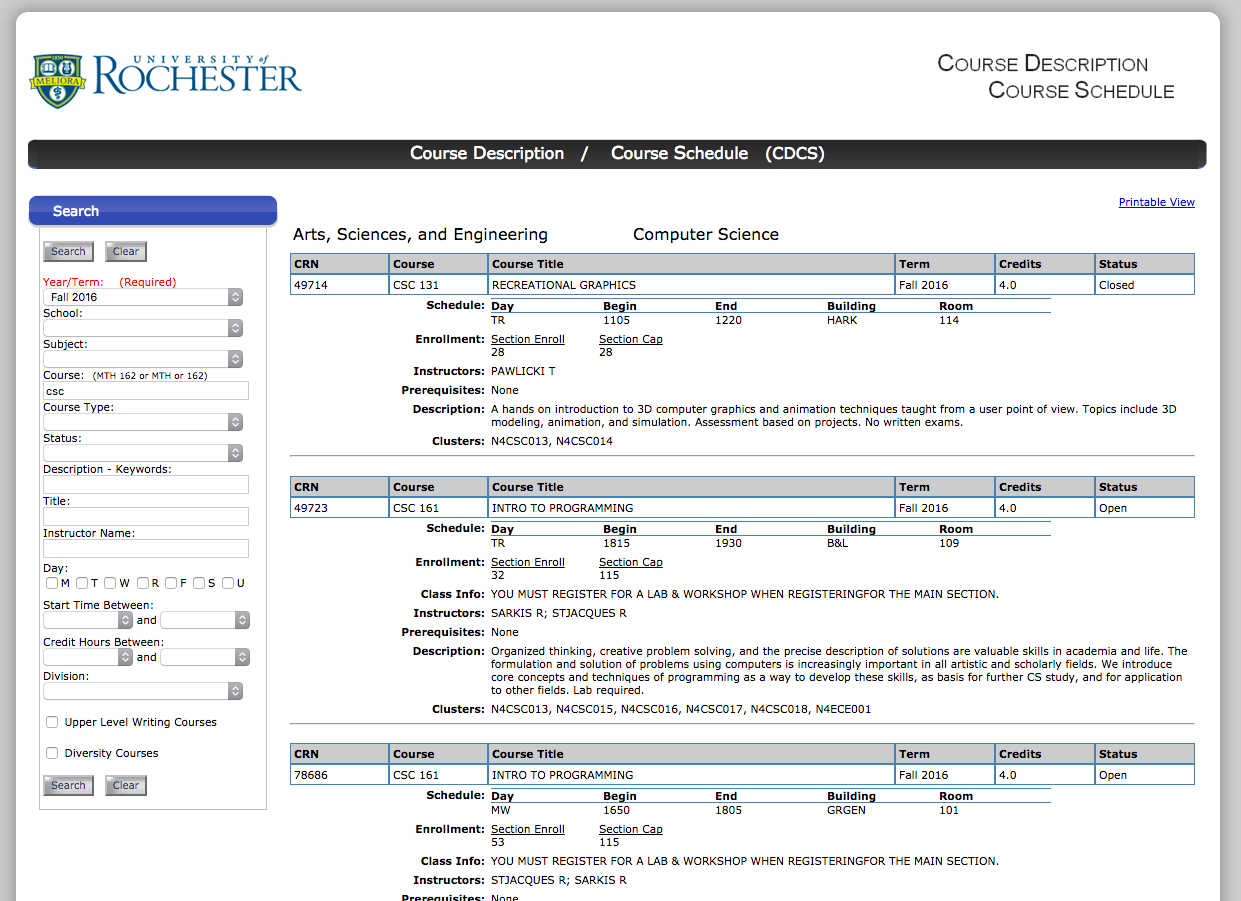
\includegraphics[width=1.00\textwidth]{images/cdcs/index}
            }
            \caption{CDCS, with the search query {\tt csc}}
            \label{fig:cdcs-index}
        \end{subfigure}\\
        \vspace{10pt}\\
        \begin{subfigure}[h]{14cm}
            \centering
            \fbox{
                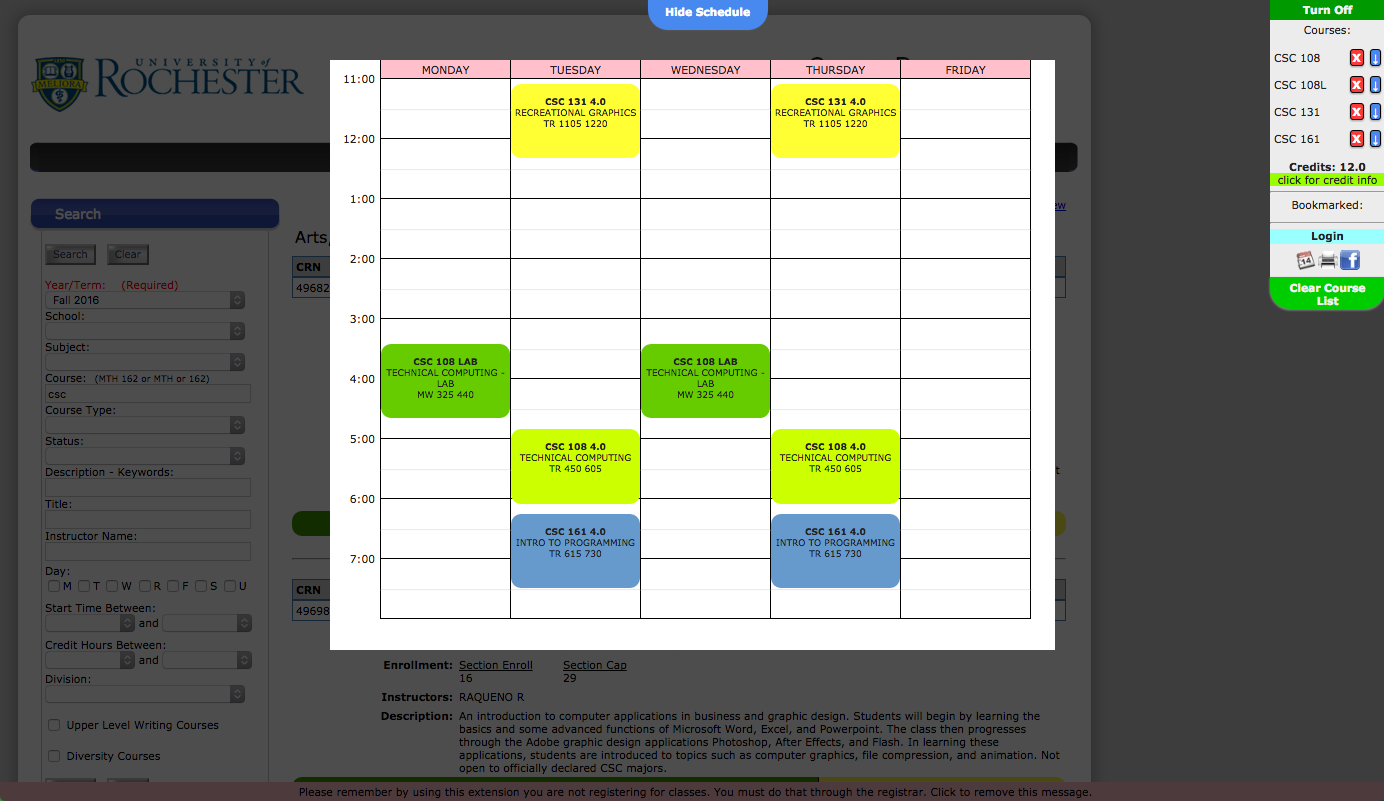
\includegraphics[width=1.00\textwidth]{images/cdcs/better}
            }
            \caption{Better CDCS, a separate browser extension that embeds buttons into the CDCS course results interface, allowing users to add courses to a locally-stored schedule}
            \label{fig:cdcs-better}
        \end{subfigure}
    \caption{CDCS and Better CDCS in their current states}
\end{figure}


``Course Description / Course Schedule,'' (or \emph{CDCS} for short) is the University's official tool for browsing the course catalog \cite{cdcs}. The CDCS interface consists of fields on the left side for inputting a search, and search results on the right side (see Figure \ref{fig:cdcs-index}). Despite ``Course Schedule'' being in its name, CDCS does not offer scheduling functionality. Course times can only be viewed, and it is up to the user to keep track of courses considered for the next semester.

\subsection{``Better CDCS''}

\emph{Better CDCS} \cite{better-cdcs} is a browser extension, available for Firefox, Safari, and Chrome, that offers a solution to the lack of scheduling mentioned above. It works by injecting ``Add Section'' and ``Bookmark Section'' buttons into the existing CDCS interface, and providing a tab on top of the screen that will toggle between the user's schedule and the search results (see Figure \ref{fig:cdcs-better}).

%%%

\section{Overview of Skedge}

\begin{figure}[H]
    \centering
    \fbox{
        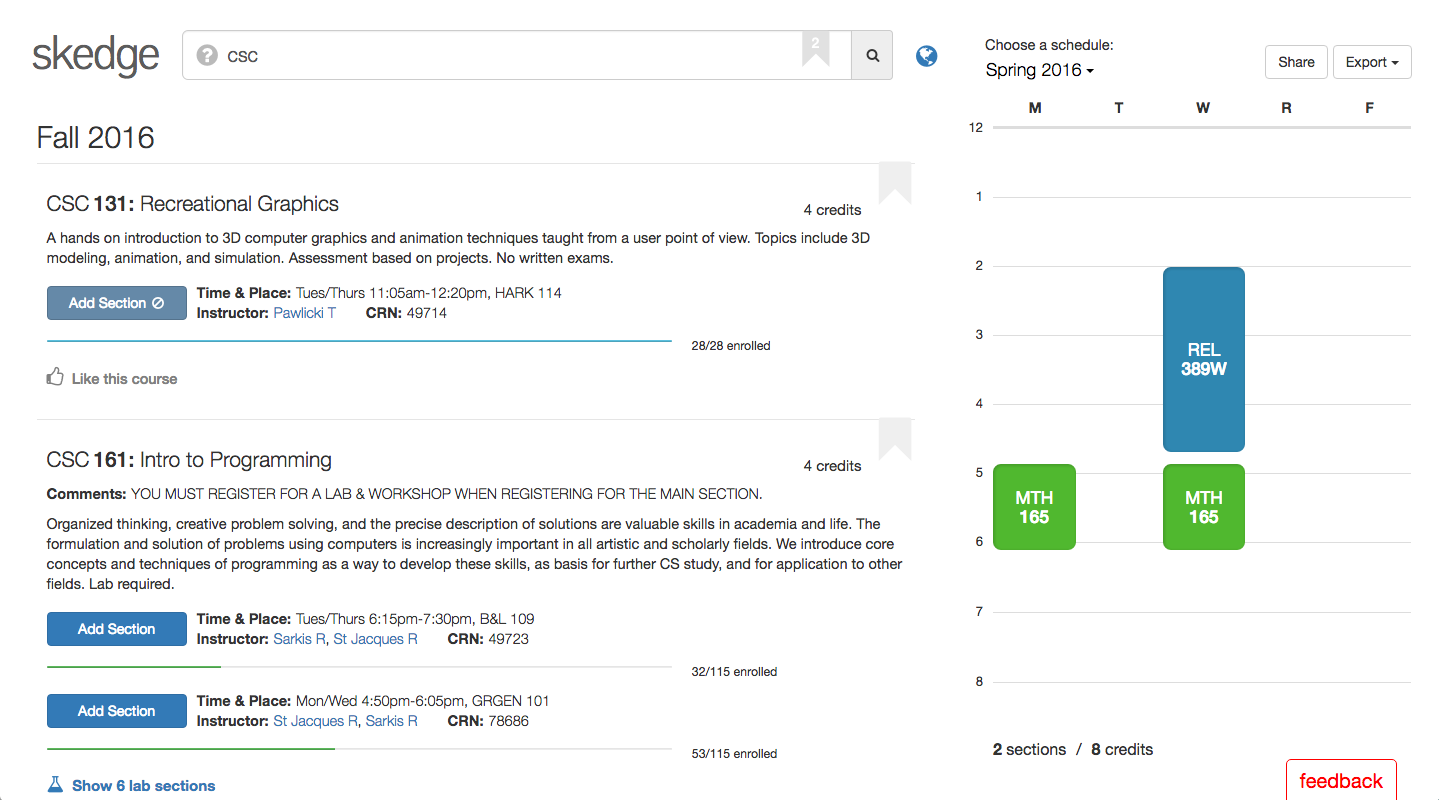
\includegraphics[width=1.00\textwidth]{images/skedge/index}
    }
    \caption[Skedge with the search query {\tt csc}]{Skedge with the search query {\tt csc} and the user's current schedule on the right}
    \label{fig:sk-index}
\end{figure}

\emph{Skedge} \cite{skedge} is, in short, CDCS combined with Better CDCS on a single platform (see Figure \ref{fig:sk-index}). Like CDCS, it is lightweight, service-oriented, and doesn't require login, but unlike Better CDCS, it also doesn't require a separate browser extension.

It matches feature-for-feature with the two tools (search options, information displayed, scheduling and bookmarks, etc.), and aims to improve upon the work of both on several fronts, which will be investigated in this paper in great detail. It is my contention that students, parents, faculty, staff, and administration can all benefit from such improvements.

\vspace{30pt}

\noindent
This paper is organized in two parts, with a brief intermission in between. First, I will explain many of Skedge's design decisions in relation to what I call my ``grievances'' with CDCS in its current state. The second part will look at collected data, extrapolating how students use Skedge and using several novel metrics to measure its usability and effectiveness as a platform.